\documentclass{article}
\usepackage{graphicx}
\usepackage[margin=1.5cm]{geometry}
\usepackage{amsmath}

\begin{document}

\title{Navigation Activity: Travel from McMurdo Station to ARIANNA}
\date{\today}
\author{Prof. Jordan C. Hanson}

\maketitle

\section{Introduction}

Observe the map below of the region surrounding McMurdo station on Ross Island near Mount Erebus, and Moore's Bay, the location of ARIANNA.  There are mountains, glaciers, and everywhere that does not have a mountain or a glacier is the frozen ocean of the Ross Ice Shelf.

\begin{figure}[ht]
\centering
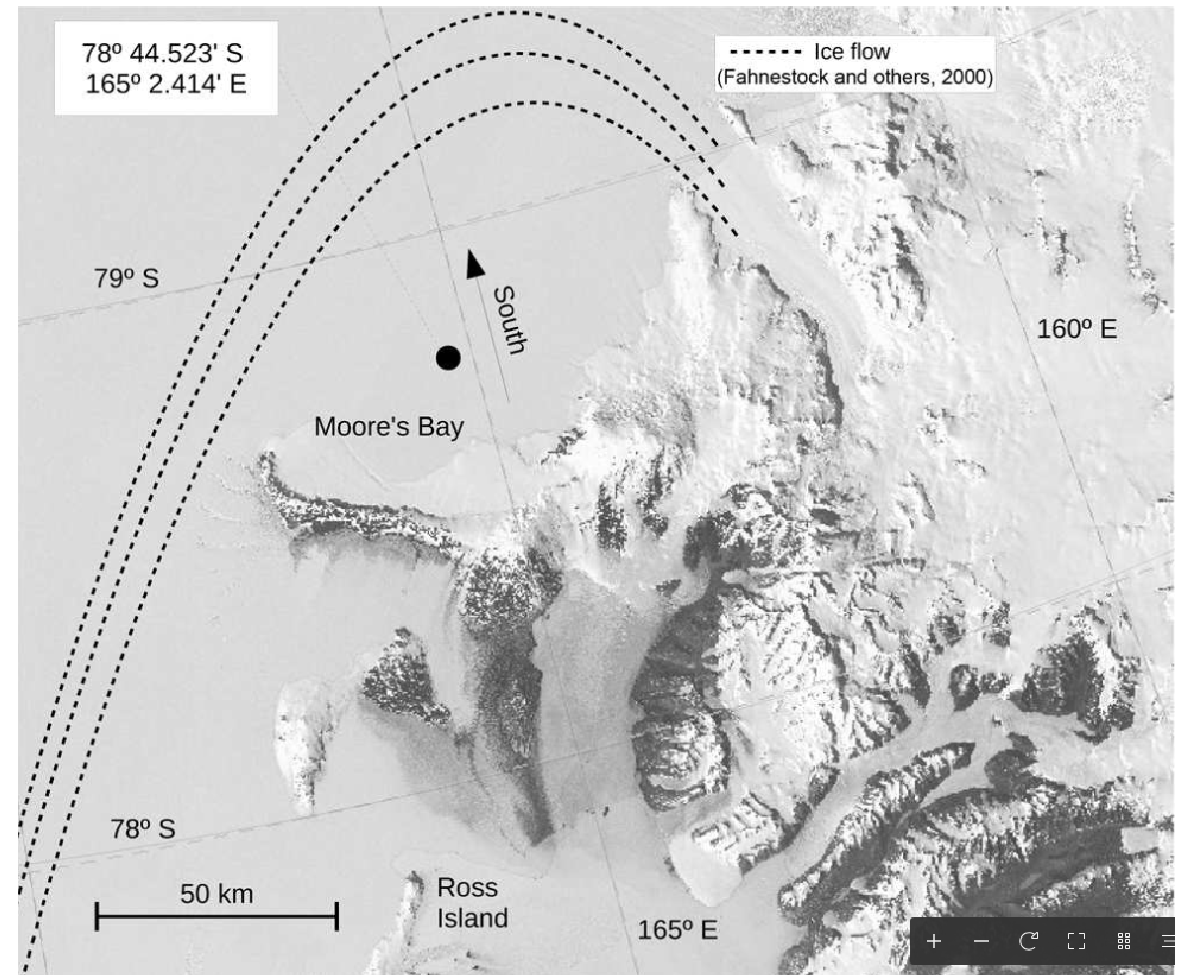
\includegraphics[width=0.5\textwidth]{NavigationMazePlain.pdf}
\caption{\label{fig:maze1} A map of the McMurdo-Moore's Bay Area.}
\end{figure}

\textbf{Our task is to navigate from Ross Island to Moore's Bay.  The starting conditions are:}
\begin{enumerate}
\item The starting point is Ross Island, and the goal is the black circle in Moore's Bay.
\item We have 1000 kg of fat-based pemmican (9 kcal/g).  We must pull it, and consume it for energy.
\item The friction coefficient depends on the area of the map.
\item Assume that we consume 2000 kcal per day automatically.
\item Assume we can travel 20 km per day in a straight line, in any direction.
\item Assume we consume an additional energy $W$, equal to the work we do on a particular 10 km line segment.
\item There are food depots already in the field, and each is work 20 MJ of energy (assume it is pemmican).
\item There are two people in our party, plus some number of dogs capable of pulling whatever load we have left.
\item For now, we neglect what food the dogs require.
\item At the end of each line segment, tally what food remains in the load, plus any food gained at a depot.  Calculate the new mass.
\end{enumerate}

Your job in this activity is to chart a course that successfully gets our two-person party, plus our super-dogs, to the black circle in Moore's Bay without starving!

\section{The Detailed Map}

\begin{figure}[ht]
\centering
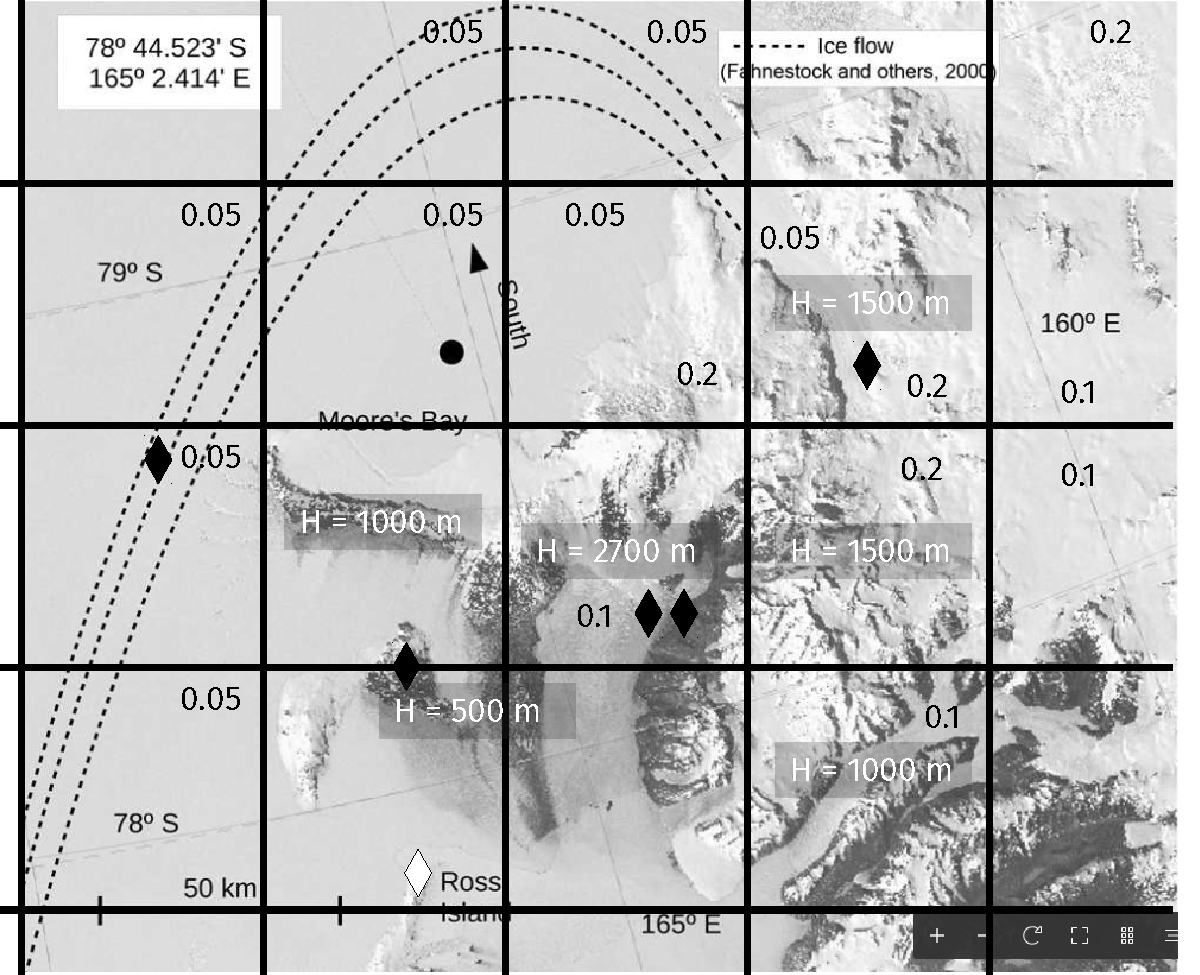
\includegraphics[width=0.5\textwidth]{NavigationMaze.pdf}
\caption{\label{fig:maze1} A map of the McMurdo-Moore's Bay Area, including food depots, elevations, and friction coefficients.  Each block is 50 km by 50 km.  The black diamonds are food depots, each work 20 MJ.  The starting point is the white diamond, and the finishing point is the black circle.  The friction coefficients are the black numbers, and they apply to the whole square.}
\end{figure}

\textbf{Write your plan below, including calculations for each line segment.}  Good luck and don't die.

\end{document}
